\documentclass[12pt]{article}
\usepackage[a4paper,margin=25mm]{geometry}
\usepackage{fontspec}
\setmainfont{TeX Gyre Termes}
\usepackage{amsmath,booktabs,graphicx,microtype,url,xurl}
\usepackage{unicode-math}
\setmathfont{TeX Gyre Termes Math}
\usepackage[section]{placeins}
\usepackage[hidelinks]{hyperref}
\usepackage[numbers,sort&compress]{natbib}
\usepackage{docmute}
\usepackage{xparse}
\setlength{\emergencystretch}{2em}
\graphicspath{{../../../results/figures/}}
\newcommand{\RXXIIIReservedTasks}{96}
\newcommand{\RXXIIISpecs}{71}
\newcommand{\RXXIIIDetectable}{64}
\newcommand{\RXXIIILift}{44.39\%}
\newcommand{\RXXIIIP}{1.65e-19}
\newcommand{\RXXIVReservedTasks}{68}
\newcommand{\RXXIVSpecs}{141}
\newcommand{\RXXIVDetectable}{115}
\newcommand{\RXXIVReplays}{306}
\newcommand{\RXXIVLift}{44.33\%}
\newcommand{\RXXIVP}{8.29e-35}
\newcommand{\PublicRepoCount}{3}
\newcommand{\PublicMainlineCommits}{265}
\newcommand{\PublicModifiedSkills}{4058}

\newcommand{\STVRArticleTitle}{From Skill-Level to Predicate-Level: Budgeted Regression Test Selection for Evolving LLM Agent Skills}
\newcommand{\STVRRunningTitle}{Predicate-Level Regression Testing for LLM Agent Skills}
\newcommand{\STVRArticleType}{Research Paper}
\newcommand{\STVRTargetJournal}{Software Testing, Verification and Reliability}
\newcommand{\STVRAuthorNames}{Liang Song\textsuperscript{1,*} and Zhai Jiabao\textsuperscript{2}}
\newcommand{\STVRPDFAuthors}{Liang Song; Zhai Jiabao}
\newcommand{\STVRAuthorNamesForTOC}{Liang Song* and Zhai Jiabao}
\newcommand{\STVRAffiliations}{%
  \textsuperscript{1}Business School, Xi'an International University,
  Xi'an 710077, China\\[0.4em]
  \textsuperscript{2}School of Management and Economics, North China
  University of Water Resources and Electric Power, Zhengzhou 450046, China}
\newcommand{\STVRAuthorEmails}{Liang Song:
  \href{mailto:liangsong_1976@126.com}{liangsong\_1976@126.com};\\[-0.1em]
  Zhai Jiabao:
  \href{mailto:zhaijiabao123@126.com}{zhaijiabao123@126.com}.}
\newcommand{\STVRCorrespondence}{Liang Song, Business School, Xi'an
  International University, Xi'an 710077, China. Email:
  \href{mailto:liangsong_1976@126.com}{liangsong\_1976@126.com}. ORCID:
  \href{https://orcid.org/0009-0002-6109-0639}{0009-0002-6109-0639}.}

\newcommand{\STVRRepositoryLink}{\url{https://github.com/ls680/predicate-impact-agent-skill-regression-testing}}
\newcommand{\STVRArchiveDOI}{10.5281/zenodo.22824889}
\newcommand{\STVRArchiveLink}{\href{https://doi.org/10.5281/zenodo.22824889}{doi:\STVRArchiveDOI}}

\newcommand{\STVRFundingStatement}{This research received no specific grant
  from any funding agency in the public, commercial, or not-for-profit sectors.}
\newcommand{\STVRConflictStatement}{The authors declare that they have no
  competing interests.}
\newcommand{\STVRAcknowledgements}{The authors have no acknowledgements to report.}
\newcommand{\STVRCreditStatement}{Liang Song: Conceptualization, methodology,
  software, validation, formal analysis, investigation, data curation,
  visualization, writing---original draft, writing---review and editing, and
  project administration. Zhai Jiabao: Methodology, validation, and
  writing---review and editing. Both authors approved the final manuscript.}
\newcommand{\STVRAIStatement}{During the preparation of this work, the authors
  used OpenAI Codex to assist with research-design iteration, code development,
  reproducibility packaging, language editing, and manuscript formatting. The
  authors reviewed and verified the generated code and text, reran the released
  integrity checks, evaluated every reported claim against the underlying
  results, and take full responsibility for the manuscript and the integrity of
  the reported results. OpenAI Codex is not an author and did not receive
  attribution as one.}


\hypersetup{
  pdftitle={\STVRArticleTitle},
  pdfauthor={\STVRPDFAuthors},
  pdfsubject={Research Paper submitted to Software Testing, Verification and Reliability},
  pdfkeywords={LLM agents, agent skills, regression test selection, change-impact analysis, dynamic coverage, mutation testing}
}

\title{\STVRArticleTitle}
\author{\STVRAuthorNames}
\date{}

\renewcommand{\maketitle}{%
  \hypersetup{pageanchor=false}%
  \begin{titlepage}
    \centering
    {\Large\bfseries \STVRArticleTitle\par}
    \vspace{1.2cm}
    {\large \STVRAuthorNames\par}
    \vspace{0.8cm}
    {\STVRAffiliations\par}
    \vspace{1.2cm}
    \begin{minipage}{0.88\textwidth}
      \setlength{\parskip}{0.6em}
      \textbf{Correspondence:} \STVRCorrespondence

      \textbf{Short running title:} \STVRRunningTitle

      \textbf{Article type:} \STVRArticleType

      \textbf{Target journal:} \STVRTargetJournal

      \textbf{Statements and declarations:} Acknowledgements, author
      contributions, funding, competing interests, data availability, ethics,
      consent, and generative-AI assistance are reported after the references.
    \end{minipage}
    \vfill
    {Prepared for initial free-format submission, September 2026\par}
  \end{titlepage}
  \hypersetup{pageanchor=true}%
  \setcounter{page}{1}%
  \markboth{\STVRRunningTitle}{\STVRRunningTitle}
}

% The source English manuscript remains unchanged. This environment discards
% its original 263-word abstract and emits the STVR-compliant abstract instead.
\RenewDocumentEnvironment{abstract}{+b}{%
  \begin{center}\bfseries Abstract\end{center}
  \begin{quotation}
    \noindentReusable skills let language-model agents retain procedures without updating model weights, but revisions create a regression-testing problem because native interactive tests are expensive. We ask whether change impact can be localized inside a skill. PredicateImpact maps a structured skill change to an action predicate, such as an object binding, destination, device, or focus target, and prioritizes historical passing tasks whose traces covered it. The method was developed on exposed ALFWorld and ScienceWorld tasks and evaluated unchanged on two disjoint, content-blind rosters. In the first confirmation, it detects all 64 killable predicate-deletion changes within a three-task budget, versus a 55.61\% conditional expectation for skill-family random selection (44.39-point lift; one-sided exact $p=1.65\times10^{-19}$). A second roster evaluates deletion, same-kind argument substitution, and adjacent-order swaps: all 115 killable changes are detected, versus 55.67\% for the same baseline (44.33-point lift; $p=8.29\times10^{-35}$). Every operator stratum and both environments pass frozen gates; 491 native replays have exact initial-state matches and no technical failures. Random ordering within the same exact predicate-coverage set ties PredicateImpact, showing that coverage granularity, rather than a complex ranking rule, explains the gain. Positive mean lift remains after dropping 50\% of true coverage edges and adding 20\% false edges. An audit of three pinned public Agent Skill repositories finds deletion-, replacement-, and relocation-shaped edits, but not verified faulty commits. Claims are therefore limited to budgeted detection on the released mutation benchmark; production-update generalization remains open.


  \end{quotation}
}{}

% STVR places acknowledgements and declaration material after the references
% and before any appendices.
\let\STVROriginalBibliography\bibliography
\renewcommand{\bibliography}[1]{%
  \STVROriginalBibliography{#1}%
  \section*{Acknowledgements}
\STVRAcknowledgements

\section*{Author Contributions}
\STVRCreditStatement

\section*{Funding}
\STVRFundingStatement

\section*{Competing Interests}
\STVRConflictStatement

\section*{Data Availability Statement}
The data and artifacts supporting the findings of this study are openly
available in Zenodo, version 1.0.0 \citep{song2026predicateimpactdataset}, at
\STVRArchiveLink. The archived
\texttt{predicate\_rts\_reproducibility\_bundle.tar.gz} has SHA-256:
\nolinkurl{3fb1dcd3d0e73e4f575d20da46ae60dabc2020c626b2bc9f302f9699c6675229}.
The corresponding source repository is available at \STVRRepositoryLink. The
version DOI and checksum identify the exact review artifact. Third-party
ALFWorld and ScienceWorld assets are excluded, with upstream identifiers and
integrity checks provided instead.

\section*{Ethics Approval and Consent}
This study evaluates software artifacts and public software benchmarks and does
not involve human participants, animals, clinical data, or personally
identifiable information. Ethics approval, consent to participate, and consent
for publication are therefore not applicable.
%
}

\begin{document}
\pagestyle{myheadings}
\sloppy
\documentclass[10pt]{article}
\usepackage[a4paper,margin=21mm]{geometry}
\usepackage{amsmath,amssymb,booktabs,graphicx,microtype,url}
\usepackage[section]{placeins}
\usepackage[hidelinks]{hyperref}
\usepackage[numbers,sort&compress]{natbib}
\setlength{\emergencystretch}{2em}
\graphicspath{{../../../results/figures/}}
\newcommand{\RXXIIIReservedTasks}{96}
\newcommand{\RXXIIISpecs}{71}
\newcommand{\RXXIIIDetectable}{64}
\newcommand{\RXXIIILift}{44.39\%}
\newcommand{\RXXIIIP}{1.65e-19}
\newcommand{\RXXIVReservedTasks}{68}
\newcommand{\RXXIVSpecs}{141}
\newcommand{\RXXIVDetectable}{115}
\newcommand{\RXXIVReplays}{306}
\newcommand{\RXXIVLift}{44.33\%}
\newcommand{\RXXIVP}{8.29e-35}
\newcommand{\PublicRepoCount}{3}
\newcommand{\PublicMainlineCommits}{265}
\newcommand{\PublicModifiedSkills}{4058}


\title{From Skill-Level to Predicate-Level: Budgeted Regression Test Selection for Evolving LLM Agent Skills}
\author{Anonymous Authors}
\date{Anonymous manuscript, September 2026}

\begin{document}
\maketitle

\begin{abstract}
Reusable skills let language-model agents retain procedures without updating model weights, but every skill revision creates a regression-testing problem. Native interactive tests are expensive, and rerunning all cases associated with a modified skill can delay feedback. We study whether change impact can be localized inside a skill. PredicateImpact maps a structured skill change to action predicates such as an object binding, destination, device, or focus target, then prioritizes historical passing tasks whose traces covered that predicate. The method was developed on previously exposed ALFWorld and ScienceWorld tasks and evaluated on two disjoint, content-blind rosters. In the first confirmation, it detects all 64 killable predicate-deletion changes within a three-task budget, compared with a 55.61\% conditional expectation for skill-family random selection (absolute lift 44.39 points, one-sided exact $p=1.65\times10^{-19}$). A second roster tests deletion, same-kind argument substitution, and adjacent-order swaps: all 115 killable changes are detected, compared with 55.67\% for the same strong baseline (lift 44.33 points, $p=8.29\times10^{-35}$). All three operator strata and both environments pass frozen gates; 491 native replays have exact initial-state matches and no technical failures. The method ties random ordering within the same exact predicate-coverage set, showing that coverage granularity, not a complex ranking rule, explains the gain. A post-hoc noise analysis retains positive mean lift even after dropping 50\% of true coverage edges and adding 20\% false edges. An audit of three pinned public Agent Skill repositories establishes that deletion, replacement, and relocation-shaped edits occur in practice, but does not substitute for real faulty commits. Claims are therefore limited to budgeted detection on the released mutation benchmark; production-update generalization remains open.
\end{abstract}

\noindent\textbf{Keywords:} LLM agents; agent skills; regression test selection; change-impact analysis; dynamic coverage; mutation testing

\section{Introduction}
Agent skills are persistent procedures, instructions, scripts, and resources that extend a language-model agent without changing its base weights. Recent systems acquire skills from trajectories, revise them continually, compose them across tasks, and govern their admission to a shared library \citep{ye2026mce,lei2026skillevolbench,gao2026skillaudit,song2026skillops}. Persistence creates a familiar software-maintenance obligation: after a skill changes, previously passing behaviors must be checked again. Unlike an ordinary unit test, however, an interactive agent test may invoke a model, launch a simulator, consume external services, or execute a long sequence of tools. Immediate full-suite replay can therefore be slow and costly.

The closest agent-skill systems already recognize this problem. SkillAudit compares paired trajectories before accepting or rolling back an update \citep{gao2026skillaudit}; SkillOps represents contracts and validation state \citep{song2026skillops}; SkillFuzz searches skill compositions under a query budget \citep{hu2026skillfuzz}. Most directly, FRAMES first samples historical cases associated with the modified skill and then adds category-stratified coverage \citep{wang2026frames}. Consequently, ``test the modified skill first'' is not a new contribution. The unresolved granularity question is whether all cases associated with one skill should remain equally likely when a revision changes only one condition, object binding, destination, or tool step.

Classical regression test selection answers an analogous question by linking program changes to prior test coverage \citep{rothermel1996rts}. Applying the idea to Agent Skills is not automatic. Skills are frequently natural-language documents rather than source modules; traces can contain aliases and environment-specific actions; a syntactic change need not affect behavior; and test outcomes are costly and sometimes nondeterministic. A useful evaluation must also avoid a common shortcut: tuning a selector on the same tasks used to claim significance.

We formulate budgeted Agent Skill regression testing around a structured action-predicate layer. A passing trace is mapped to predicates such as \texttt{take\_object=apple}, \texttt{place\_destination=drawer}, or \texttt{focus\_object=thermometer}. Given a parent--child skill change localized to one predicate, PredicateImpact first runs tasks that previously covered that predicate, then other cases for the same skill family. This is a lightweight dynamic change-impact analysis; it needs no model training and can consume traces already produced by a release gate.

The investigation deliberately preserves failed paths. Coarse operation-level mutations were dense within a skill family, so knowing exact operation coverage added little or nothing over skill-family random selection. We advanced to predicate-level changes only after writing a fixed sparse-specification rule on exposed development data. The rule and selector were then applied unchanged to a first content-blind roster. After that confirmation, a second question---operator transfer---was frozen before a disjoint roster was opened and tested three edit operators.

This paper makes four contributions:
\begin{itemize}
  \item a predicate-level dynamic change-impact formulation for selecting historical Agent Skill tests under a fixed interaction budget;
  \item an auditable mutation benchmark over native ALFWorld and ScienceWorld execution, with outcome-blind development, two disjoint content-blind rosters, exact initial-state checks, and input hashes;
  \item evidence that predicate coverage, rather than within-coverage ranking, raises killable-change detection by about 44 percentage points over a FRAMES-style skill-family baseline in both confirmations;
  \item explicit external-validity checks: three mutation operators, a coverage-noise grid, an audit of pinned public \texttt{SKILL.md} histories, and negative results for family-dense changes.
\end{itemize}

We ask: \textbf{RQ1} Does predicate-level coverage improve early detection over skill-level association? \textbf{RQ2} Does the effect transfer from action deletion to argument substitution and action-order changes, across both environments? \textbf{RQ3} Which component explains the gain, and how sensitive is it to incomplete or spurious historical coverage? The unit of evidence is a frozen mutation specification, not an LLM family or a production commit.

\section{Related Work}
\paragraph{Skill evolution and governance.}
Meta Context Engineering, AlignEvoSkill, SkillHone, SkillEvolBench, and ContinualSkillBench study acquisition, refinement, persistent decision history, or longitudinal evaluation of procedural skills \citep{ye2026mce,wang2025alignevoskill,li2026skillhone,lei2026skillevolbench,guan2026continualskillbench}. SkillCAT combines contrastive evidence and topology-aware merging, while SkillAudit uses paired execution evidence to reject or roll back harmful updates \citep{chen2026skillcat,gao2026skillaudit}. SkillOps treats the library as a maintained software ecosystem with typed contracts and validation state \citep{song2026skillops}. These systems motivate continuous regression evidence, but they do not make every test attached to a skill equally informative.

FRAMES is the nearest testing-policy baseline. Its regression pool gives priority to cases associated with skills modified in the current iteration and supplements them with stratified random cases \citep{wang2026frames}. Our skill-family random baseline gives the selector the same modified-skill information. PredicateImpact asks whether historical dynamic coverage inside that family can localize a smaller impact set. SkillFuzz instead searches compositions for implicit intents using extracted contracts and a differential oracle \citep{hu2026skillfuzz}; its search unit, threat model, and execution-free first stage differ from post-update regression selection.

\paragraph{Regression test selection.}
Regression test selection reuses tests from an existing suite and selects those relevant to a modified program. Established evaluation criteria include inclusiveness, precision, efficiency, and safety \citep{rothermel1996rts}. Dynamic approaches record which program entities a passing test executes and rerun tests covering changed entities. PredicateImpact transfers this design pattern to the procedural layer of an Agent Skill, where the covered entity is an action predicate rather than a source statement or method. We do not claim classical RTS concepts as novel; the contribution is their operationalization and controlled evaluation for evolving agent skills.

\paragraph{Mutation and interactive benchmarks.}
ALFWorld aligns text interaction with embodied household tasks, while ScienceWorld supplies procedurally generated science tasks and gold action sequences \citep{shridhar2021alfworld,wang2022scienceworld}. Mutation testing supplies controlled faults when naturally occurring failing revisions are scarce. This improves causal localization but can favor coverage-based methods, so operator diversity, equivalent-mutant accounting, strong baselines, and real-change audits are necessary. Our public-history audit uses pinned repositories from Anthropic, OpenAI, and Microsoft only to check whether corresponding edit shapes occur \citep{anthropicskills2026,openaiskills2026,microsoftskills2026}; it does not label those edits as defects.

\section{Problem Formulation}
Let $T=\{t_1,\ldots,t_n\}$ be historical tests. Each task $t_i$ belongs to a skill family $g_i$, has a previously passing action trace $\tau_i=(a_{i1},\ldots,a_{im})$, and has observed execution cost $c_i$. A deterministic parser $\phi$ maps an action to either an action predicate $p=(k,v)$ or no predicate. The dynamic coverage matrix is
\begin{equation}
 C_{ip}=\mathbb{1}\left[\exists a\in\tau_i:\phi(a)=p\right].
\end{equation}
A structured update descriptor is $\delta=(g,p)$: skill family $g$ changed at predicate $p$. In a deployed system, $\delta$ can come from a typed skill diff, an author annotation, or a parser over a structured procedure. This paper evaluates the case in which $\delta$ is available; automatic localization from arbitrary prose is outside scope.

Executing the updated skill on $t_i$ yields binary failure indicator $Y_i(\delta)$. A change is \emph{killable} by the available suite if $\max_i Y_i(\delta)=1$. Given budget $B$, a selector returns an ordered subset $S_B(\delta)$, and detects the change when
\begin{equation}
 D_B(\delta)=\mathbb{1}\left[\max_{t_i\in S_B(\delta)}Y_i(\delta)=1\right].
\end{equation}
The primary endpoint is mean $D_3$ among killable changes. We also report an all-mutation score that includes changes surviving every available test. A surviving change may be behavior-preserving or may expose a test-suite weakness; it cannot be relabeled as detected.

The practical comparison is skill-level association: once $g$ is known, choose $B$ cases uniformly from that family. Conditional on a fixed family containing $N$ tests and $K$ failing tests, its exact detection probability is
\begin{equation}
 q(N,K,B)=1-\frac{\binom{N-K}{\min(B,N)}}{\binom{N}{\min(B,N)}}.
\end{equation}
This baseline is stronger than global random sampling because it receives the changed skill identity.

\section{PredicateImpact}
\subsection{Predicate extraction}
The fixed parser recognizes nine predicate types. ScienceWorld contributes focus target, activated device, picked-up object, and colored-box destination. ALFWorld contributes taken object, placement destination, transformation device, opened target, and used device. Numeric instance suffixes and inventory aliases are normalized. The parser is intentionally small and inspectable; no language model or outcome label is used to construct coverage.

\begin{table}[t]
\centering
\caption{Fixed action predicates used for historical dynamic coverage.}
\label{tab:predicates}
\begin{tabular}{lll}
\toprule
Environment & Predicate type & Example value \\
\midrule
ALFWorld & take object & apple \\
ALFWorld & place destination & drawer \\
ALFWorld & transform device & sink basin \\
ALFWorld & open target / use device & safe / desk lamp \\
ScienceWorld & focus object & thermometer \\
ScienceWorld & activate device & thermometer \\
ScienceWorld & pickup object & wire \\
ScienceWorld & box destination & blue box \\
\bottomrule
\end{tabular}
\end{table}

\subsection{Selection rule}
PredicateImpact places tasks from the modified family that covered $p$ before family tasks that did not, followed by other families. Within the covered set, the implementation prefers an occurrence with a larger downstream trace fraction and then lower healthy steps per occurrence. Formally, for the first matching index $j_i$ in a trace of length $m_i$, the covered-task priority contains
\begin{equation}
 r_i=\left(-\frac{m_i-j_i}{m_i},\frac{c_i}{\#\{a\in\tau_i:\phi(a)=p\}}\right).
\end{equation}
Stable task identifiers break ties. The full suite remains available if the budget expands; the method changes order rather than deleting evidence permanently.

This ranking has linear scan complexity in stored trace length plus sorting. More importantly, the experiment includes a predicate-coverage random ablation that receives the same exact covered set but randomizes its internal order. If this ablation ties PredicateImpact, the defensible contribution is coverage granularity, not $r_i$.

\subsection{Baselines}
We compare with: (i) predicate-coverage random; (ii) skill-family random, the primary FRAMES-style baseline; (iii) global random; (iv) family-stratified sampling; (v) lexical similarity between the update descriptor and task objective; (vi) shortest healthy test first; and (vii) an outcome-aware oracle upper bound. Randomized methods use 200 stable seeds. Only the skill-family random baseline enters the frozen primary lift and conditional randomization test; the coverage-random ablation diagnoses the source of any gain.

\section{Experimental Design}
\subsection{Development and exposure control}
Development uses 78 previously exposed ScienceWorld and 30 exposed ALFWorld tasks. Seventy-one and 27, respectively, have successful healthy references. Before any mutation result is read, a fixed generator retains predicates covered by at least one and no more than half of the successful tasks in a family. For each family and predicate type, it keeps at most one singleton and four multi-task predicates. An initial, never-executed draft was rejected because 74 of 96 specifications were singletons; preserving it prevents silent protocol rewriting. The corrected development set contains 77 specifications, 72 of which are killable.

Development advances only if there are at least 30 killable specifications, 10 multi-task specifications, two environments, and eight skill families; detection must be at least 0.80, absolute lift over skill-family random at least 0.20, and one-sided conditional $p\leq0.01$. The final development result passes, after which the algorithm and first confirmation protocol are frozen.

\subsection{First independent confirmation}
An exposure ledger identifies task references already present in project files. Before task objectives, gold paths, or outcomes are read, SHA-256 ranking selects eight ALFWorld \texttt{valid\_unseen} cases from each of six families and 16 official ScienceWorld test variants from each of three families: 96 tasks in total. Healthy references use the ALFWorld hand-coded expert or ScienceWorld gold sequence. Five ALFWorld double-object references fail within the fixed horizon and remain in the artifact; the 91 successful references determine eligible coverage.

The development generator is applied unchanged, producing \RXXIIISpecs{} deletion specifications and 185 native replays. The first confirmation repeats the development gates and additionally requires each environment to attain detection at least 0.75, lift at least 0.15, and one-sided $p\leq0.05$. No threshold changes are allowed after opening the roster.

\subsection{Operator-transfer confirmation}
R24 is designed after observing R23, so it is a new confirmation question rather than a preregistered replication. All code, three operators, sampling, endpoints, and gates are nevertheless frozen before the second roster's content is opened. The roster contains all 32 compatible ALFWorld cases remaining after R23 and a content-blind sample of 12 unused ScienceWorld test variants per family. It has 68 tasks, zero overlap with R23, and 68 successful references.

Each base predicate expands into three operators when applicable:
\begin{enumerate}
  \item \textbf{deletion}: remove the first matching action;
  \item \textbf{argument substitution}: replace it with a different historically admissible action of the same predicate kind;
  \item \textbf{adjacent-order swap}: exchange the matching action with its successor.
\end{enumerate}
Applicability is derived only from the healthy trace. The frozen artifact has 141 operator specifications and 306 planned native replays. The gate requires at least 30 killable specifications, all three operators, both environments, and six families; overall detection must be at least 0.75, lift at least 0.15, and $p\leq0.01$. Each operator must contribute at least six killable specifications, detection at least 0.65, and lift at least 0.10.

\subsection{Native execution and audit}
Every mutated trace is executed in the native environment from a fresh reset. A hash of initial observation, objective, and admissible actions must match the healthy reference. Environment exceptions are recorded as technical errors and are never counted as mutation kills. ScienceWorld uses a pinned upstream simulator JAR; task split membership is checked at collection time. The experiment ran with a 20-core container quota and 90~GiB memory limit on an AMD EPYC~7642 host. An RTX~3090 was present but unused because these confirmation experiments perform no model inference. The 164 independent-roster references and 491 mutation replays required about 22.1 summed episode-minutes.

Each run specification hashes code, configuration, roster, simulator, healthy traces, and upstream implementation. An audit resolves paths inside the project root, checks every input hash, verifies the original source tree, and rejects any task outside the frozen roster. The two confirmation runs produce exact initial-state matches for all 491 replays and zero technical failures.

\subsection{Statistical scope}
For each killable specification, the family-random detection probability is computed exactly using the hypergeometric complement above. Independent randomized selection per specification induces a Poisson-binomial null distribution; the reported one-sided $p$ is its upper-tail probability at PredicateImpact's observed number of detections. It tests the randomized selection mechanism conditional on the frozen benchmark. It is not population inference over future skills, task families, repositories, or mutation operators. Environment and operator strata are reported separately, and the frozen gates avoid choosing a favorable subgroup after inspection.

\section{Results}
\subsection{RQ1: Predicate coverage improves early detection}
Table~\ref{tab:main} reports both confirmations. PredicateImpact detects every killable specification within three tasks. In R23, the detection rate is 1.000 versus a 0.5561 family-random expectation, an absolute lift of \RXXIIILift{} ($p=1.65\times10^{-19}$). ALFWorld lift is 0.3565 ($p=5.29\times10^{-7}$); ScienceWorld lift is 0.5164 ($p=3.12\times10^{-13}$). All ten frozen confirmation checks pass.

When all specifications enter the denominator, including seven changes not killed by any available task, the candidate's R23 mutation score is 0.9014 versus 0.5012 expected for skill-family random. Executing at most three tasks per killable update reduces test executions by 75.45\% relative to rerunning every eligible test in the modified family.

\begin{table}[t]
\centering
\caption{Independent confirmation at a three-task budget. Detection is conditioned on changes killable by the available suite; all-mutation score retains surviving changes in the denominator.}
\label{tab:main}
\resizebox{\linewidth}{!}{%
\begin{tabular}{lrrrrrrrr}
\toprule
Run & Tasks & Specs & Killable & Predicate & Family rnd. & Lift & All-mut. & Test reduction \\
\midrule
R23 deletion & 96 & 71 & 64 & 1.0000 & 0.5561 & 0.4439 & 0.9014 & 0.7545 \\
R24 three operators & 68 & 141 & 115 & 1.0000 & 0.5567 & 0.4433 & 0.8156 & 0.7132 \\
\bottomrule
\end{tabular}}
\end{table}

\begin{figure}[t]
\centering
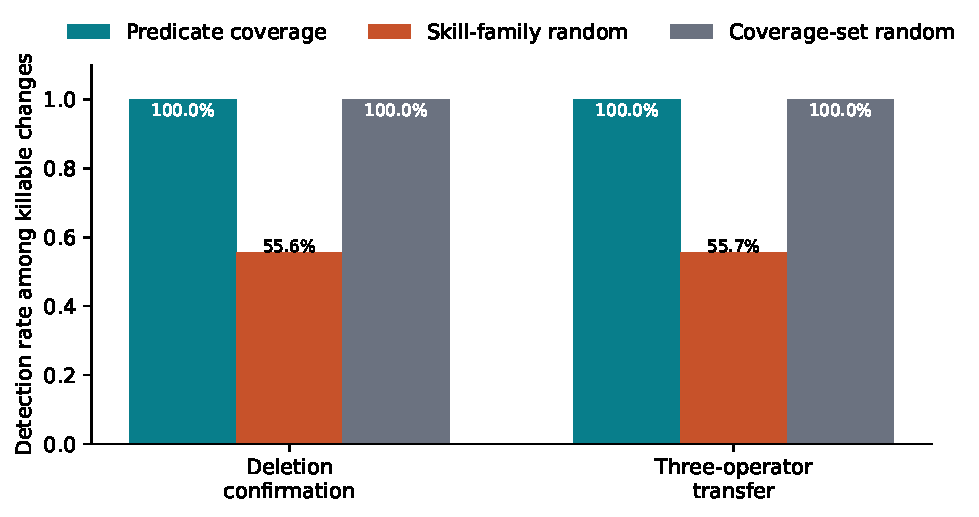
\includegraphics[width=.85\linewidth]{predicate_confirmation.pdf}
\caption{Detection among killable changes. PredicateImpact and random order within the exact predicate-coverage set tie; both outperform skill-family random.}
\label{fig:confirmation}
\end{figure}

\subsection{RQ2: The result transfers across operators and environments}
The disjoint R24 roster gives nearly the same aggregate estimate: 1.000 detection versus 0.5567, lift \RXXIVLift{}, with $p=8.29\times10^{-35}$. The ALFWorld and ScienceWorld lifts are 0.3595 and 0.5346. Table~\ref{tab:operators} shows that deletion, same-kind argument substitution, and adjacent-order swap each exceed the pre-specified per-operator threshold. The smallest stratum is order swap with 18 killable changes; even there lift is 0.4038 and conditional $p=1.16\times10^{-5}$. All ten operator-transfer checks pass.

Twenty-six of 141 R24 specifications survive every available task. Keeping them in the denominator gives an all-mutation score of 0.8156 for PredicateImpact and 0.4541 expected for family random. We do not call the survivors equivalent mutants because the available test suite cannot prove semantic equivalence.

\begin{table}[t]
\centering
\caption{R24 result by mutation operator.}
\label{tab:operators}
\begin{tabular}{lrrrr}
\toprule
Operator & Killable & Predicate & Family random & Lift \\
\midrule
Delete matching action & 58 & 1.0000 & 0.5745 & 0.4255 \\
Same-kind argument substitution & 39 & 1.0000 & 0.5120 & 0.4880 \\
Adjacent-order swap & 18 & 1.0000 & 0.5962 & 0.4038 \\
\bottomrule
\end{tabular}
\end{table}

\subsection{RQ3: Coverage granularity explains the gain}
The exact predicate-coverage random ablation also detects every killable change in both confirmations (Figure~\ref{fig:confirmation}). PredicateImpact's downstream-span and cost tie-breakers therefore contribute zero observed lift at the primary budget. Lexical similarity can sometimes recover predicate values from task text, but it does not provide the same reliable coverage guarantee; shortest-first and global policies often spend early budget outside the actual impact set. The result supports a simpler system design: record reliable predicate coverage first, and treat elaborate within-set ranking as unproven until a benchmark contains multiple covered tasks with heterogeneous failure propagation.

The early negative experiments clarify when this information is not useful. For coarse ScienceWorld operation mutations, opportunity-aware selection detects 27 of 28 killable family--operator instances, but family random already has 0.9016 expected detection (lift 0.0627, $p=0.119$). In ALFWorld it detects 31 of 33 while family random reaches 0.9727 expectation (lift $-0.0333$, $p=0.984$). If a change affects nearly every test attached to a skill, skill-level association is enough. Predicate-level coverage is valuable specifically for sparse conditional changes.

\section{Robustness and External Grounding}
\subsection{Coverage corruption}
After partial R24 logs were visible but before the run completed, we fixed a post-hoc sensitivity grid; it is not confirmatory evidence. True coverage edges are independently dropped at rates 0--0.50 and non-coverage family edges added at rates 0--0.20. For each of 20 combinations, 500 stable hash seeds reorder observed-covered tasks by healthy execution cost.

At 20\% missing and 10\% spurious edges, mean detection is 0.9478 in R23 and 0.9258 in R24, retaining lifts of 0.3918 and 0.3690. At the most severe 50\%/20\% setting, rates are 0.7695 and 0.7358, with lifts of 0.2134 and 0.1791. All 500 simulations retain positive aggregate lift in both datasets. These quantiles characterize the specified corruption mechanism, not sampling uncertainty over deployments.

\begin{figure}[t]
\centering
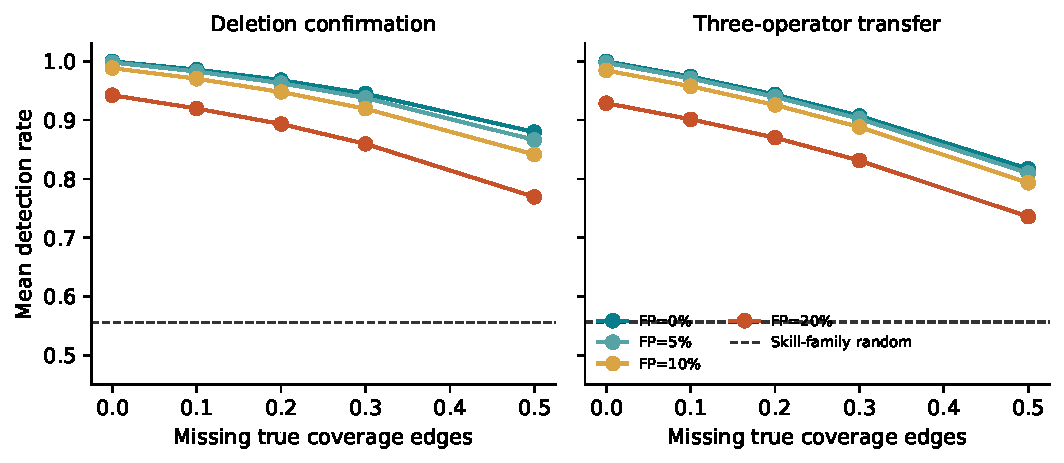
\includegraphics[width=\linewidth]{coverage_noise.pdf}
\caption{Post-hoc coverage-noise sensitivity. Dashed lines are the exact skill-family random expectations. FP denotes the spurious-edge rate.}
\label{fig:noise}
\end{figure}

\subsection{Public Skill history audit}
To test whether the operator shapes are wholly artificial, we pin the main branches of the public Anthropic, OpenAI, and Microsoft Agent Skill repositories after R24's operators were fixed \citep{anthropicskills2026,openaiskills2026,microsoftskills2026}. We traverse 265 first-parent commits. Across 120 commits that modify an existing \texttt{SKILL.md}, there are 4,058 file edits; 3,952 come from Microsoft's batch documentation synchronization, so files are not treated as independent observations.

Zero-context diff heuristics find deletion in 4,037 edits, mixed add/delete hunks in 4,028, similar-line replacement candidates in 3,835, and exact-line relocation candidates in 665. All three repositories contain deletion, replacement-shaped, and relocation-shaped edits. The audit releases commit IDs, paths, counts, and hashes but not third-party file contents. These observations ground structural edit primitives only. They neither show that a public edit was faulty nor demonstrate that PredicateImpact would select a failing production test for it.

\section{Discussion}
\paragraph{Practical interpretation.}
The actionable result is modest and useful. A release system that already records passing task traces should not attach those traces only to a whole skill. It should also record which structured conditions, object bindings, destinations, and tool steps each task exercised. When a diff identifies one such predicate, replay covered tasks before drawing broadly from the skill family. In our frozen benchmarks, this recovers all killable changes with at most three native tests while avoiding roughly 71--75\% of full-family executions.

\paragraph{What is not supported.}
The experiments do not show that downstream-span ranking is better than random ordering inside the same impact set. They do not show that free-form prose diffs can be localized automatically, that a selected test will expose every semantic consequence, or that three tests are safe for deployment. ``Detected'' means at least one available task loses successful terminal behavior under a controlled mutation. A production gate should still expand to broader stratified tests when risk, novelty, or coverage uncertainty warrants it.

\paragraph{Relation to the failed recovery study.}
This work originated in an attempt to repair contaminated descendants using lineage and counterfactual re-distillation. Controlled simulations showed cost savings, but three model families over 288 native model--task pairs produced no stable recovery benefit. Rather than tune further on those held-out outcomes, we changed the lifecycle question: after any skill update, which tests should execute first? The negative study remains in the artifact. It motivates a test-selection contribution but is not counted as positive evidence for PredicateImpact.

\section{Threats to Validity}
\paragraph{Construct validity.}
The procedural unit under mutation is a recorded successful action program. Many deployed Agent Skills are natural-language documents whose execution depends on an LLM. The benchmark therefore measures regression selection for an instrumented procedural layer, not end-to-end interpretation of arbitrary \texttt{SKILL.md} prose. Gold and expert traces eliminate executor noise but also reduce ecological complexity.

The change descriptor supplies the correct family, predicate kind, and value. Real diff localization may be ambiguous. The noise study perturbs coverage, not the change descriptor itself. Terminal success is a strong outcome for these environments, but a real system may require safety, latency, cost, or policy assertions even when a task completes.

\paragraph{Internal validity.}
Mutation locations are derived from historical coverage, which structurally favors a coverage selector. This is the standard coupling assumption behind dynamic RTS, but it can exaggerate performance if real faults propagate outside covered entities. We mitigate rather than eliminate this threat with two disjoint rosters, three operators, surviving-mutant reporting, exact state matching, and a public edit-shape audit. No technical exception is counted as a kill.

R24 was designed after R23 and confirms operator transfer, not an untouched replication of the entire research process. The coverage-noise grid was fixed after some R24 logs were visible and is explicitly post hoc. R23 remains the principal independent confirmation of the R22-developed rule.

\paragraph{Statistical and external validity.}
Conditional randomization $p$ values quantify how surprising the detections are under the specified family-random selector on these fixed changes. They do not imply random sampling from all skills. The benchmark includes two text environments, nine families in R23 and eight in R24; it excludes web, coding, multimodal, multi-agent, and live-service side effects. Public repository edit counts are heavily clustered by repository and synchronization commit. Real faulty skill revisions with linked failing tests remain the most important missing evidence.

\section{Reproducibility}
The artifact separates each research stage and preserves every failed predecessor. R22 contains the outcome-blind generator and development results. R23 and R24 contain frozen rosters, healthy trajectories, mutation specifications, raw native outcomes, selector evaluations, completion records, and independent hash audits. R25 contains pinned public-repository metadata and aggregate diff records. R26 contains the full noise grid and its timing warning. Submission tables and figures are regenerated by \texttt{analysis/regression\_submission.py}.

The core confirmation requires Python, ALFWorld 0.4.2, TextWorld 1.7.0, ScienceWorld 1.2.3 with the pinned simulator JAR, and OpenJDK 17. It does not require Docker, a GPU, model weights, or external APIs. Upstream benchmark data are not redistributed; manifests and setup scripts document their expected locations. Content hashes bind all local inputs, and the released tables retain more precision than the manuscript.

\section{Conclusion}
Budgeted regression testing for evolving Agent Skills benefits from looking inside the modified skill. Across two disjoint ALFWorld/ScienceWorld rosters, predicate-level dynamic coverage raises killable-change detection by about 44 percentage points over a strong skill-family random baseline at a three-test budget, with the effect reproduced across deletion, same-kind argument substitution, and adjacent-order swaps. The strongest ablation ties the method, locating the contribution precisely: fine-grained impact coverage matters; the proposed within-set ranking has not earned credit. Coverage noise degrades gracefully under the tested mechanism, and public histories contain corresponding edit shapes. The remaining step toward production evidence is evaluation on naturally occurring faulty skill commits with independent failing tests and automatic diff localization.

\bibliographystyle{plainnat}
\bibliography{../../references}

\appendix
\section{Frozen Gate Summary}
R23 requires minimum counts for killable and multi-task specifications, both environments, eight families, overall detection and lift, overall conditional $p$, and environment-specific detection, lift, and $p$. R24 requires minimum killable specifications, all three operators, both environments, six families, overall detection, lift, and $p$, plus minimum count, detection, and lift for every operator. Every listed check evaluates to true in the machine-readable completion files.

\section{Evidence Denominators}
R23 contains 71 specifications, of which 64 are killable; R24 contains 141, of which 115 are killable. The primary endpoint conditions on killability because no selector can detect a change that produces no failing test in the available suite. The all-mutation score retains all specifications to expose this conditioning. We report both and prohibit replacing ``killable-change detection'' with unqualified ``fault detection'' in derived claims.

\section{Exposure Timeline}
Development uses only tasks already exposed by earlier recovery experiments. The R23 roster is frozen from identifier-level inventory before its task content is opened. R24 excludes all R23 identifiers, freezes its code and roster, then collects healthy trajectories. The R25 repository snapshots are selected only after R24 operators are fixed. R26 is explicitly marked post hoc because partial R24 outcomes were visible when its noise grid was written.

\end{document}

\end{document}
